\section{Data}
\label{sec:data}

We will now present our numerical experiments, using the theory presented in~\secref{sec:segmentation} and data produced by the pipeline outlined in~\secref{sec:data}.
Specifically the U-Net model architecture is used for segmentation as previously described in~\secref{sec:unet}.
We start by describing the general experimental setup in~\secref{sec:experimental-setup}.
A comparative investigation into the suitability of the different raster data types (aerial photography and/or LiDAR DSMs) for predicting building outlines is presented in~\secref{sec:features}.
In~\secref{sec:technique-experiments} we try to determine if techniques intended to combat overfitting and aid training actually have their intended effect; specifically batch normalization, dropout, and data augmentation.
The different LiDAR normalization methods presented in \algref{alg:local-min-max-scaling} and \algref{alg:metric-normalization} are implemented and compared in~\secref{sec:normalization-experiment}.
Finally, \secref{sec:loss-experiment} presents the empirical efficiency of different surrogate loss functions.


\subsection{Coordinate Systems}
When it comes to geographical data, as with most things, different \textit{coordinate systems} have different trade-offs.
Coordinate system \textit{projections} are used in order to map a given set of coordinates to another coordinate system.
The target coordinate system might have a domain which is a proper subset of the source coordinate system, and the target system is not necessarily of the same dimensionality.
Cartographers must apply a projection in order to represent the three-dimensional spherical shape of the earth on a two-dimensional surface.
For instance, the common \textit{Mercator map projection} is suitable for navigation since a path of straight bearing is represented as a straight line on the resulting map, but the projection does \textit{not} preserve area as surfaces towards the poles become elongated \cite[p.~38]{map_projections_1987}.

A spherical coordinate system is most suitable for representing \textit{arbitrary} positions on the earths surface.
The most common coordinate system is the \textit{geographic coordinate system} (GPS).
A given point is uniquely represented by three scalars, $\vec{p} = (\phi, \lambda, z)$.
The latitude, $\phi$, is the angle between the equitorial plane and the line connecting the point to the center of the earth.
Likewise, the longitude, $\lambda$, is the angle between the same line and the reference meridian passing through Greenwich, England.
The elevation, $z$, is the radial distance from sea level to the given point.
Negative values for $z$ do not necessarily imply that the given point is below the ground, as certain areas (such as in the Netherlands) are situated below sea level.
It is therefore not sufficient to represent elevation data with unsigned floating point numbers.

Even though GPS is able to uniquely represent geographic positions with a high degree of accuracy, it is unsuitable for many applications.
For instance, cartesian transformations and norms are cumbersome to calculate, and data structures and visualizations which are fundamentally two dimensional, such as maps, rasters, and matrices, become difficult to use with a spherical coordinate system.

In order to solve this problem we define a set of coordinate system \textit{projections} which approximates given regions of the earth surface as being flat planes.
The resulting coordinate system is cartesian, and thus allows you to represent geographic points in the more common $\vec{p} = (x, y, z)$ format.
Cartesian distance norms such as $||\vec{p}_1 - \vec{p}_2||_2$ and cartesian translations $\vec{p}_1 + \vec{\Delta}$ stay within pre-defined error tolerances as long as operations are contained to the given validity region of the given projection.

\begin{figure}[H]
  \centering
  \includegraphics[width=0.6\linewidth,natwidth=443,natheight=480]{europe-utm-zones.png}
  \caption{
    The figure shows the UTM zones required in order to cover the entirety of Europe, from \texttt{29S} to \texttt{38W}.
    This public domain image has been sourced from Wikimedia \cite{wiki:europe_utm_zones}.
  }
\end{figure}


\subsection{Data types}

Geographical data can largely be divided into two sub-categories, \textit{vector data} and \textit{raster data}.
We will give a brief overview of these two data representations.

\subsubsection{Vector data}
A \textit{line string} is an ordered collection of geographic points $(\vec{p}_0, \ldots, \vec{p}_n)$ defining a path which connects each consecutive point by a straight line.
The points are therefore necessarily order dependent.
A \textit{simple} line string is a path which does \textit{not} intersect itself, while a \textit{complex} line string is one that does.
When the first and last points of a line string are identical it is considered a \textit{linear ring}, i.e.\ $l = (\vec{p}_0, \ldots, \vec{p}_n, \vec{p}_0)$.
A \textit{polygon} can therefore be represented by a simple linear ring which defines its \textit{exterior hull} and any number of simple linear strings which defines its \textit{interior hulls}.
\figref{fig:polygon-representation} illustrates these concepts for polygons with and without interior hulls. % chktex 2

\begin{figure}[htb]
  \centering
  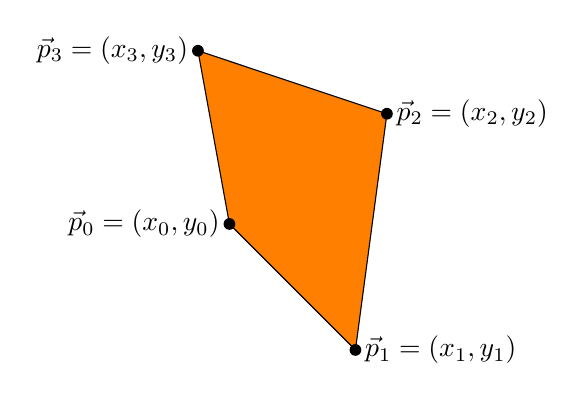
\begin{tikzpicture}[scale=2]
  \coordinate (zero) at (0, 0);
  \coordinate (one) at (0.8, -0.8);
  \coordinate (two) at (1, 0.7);
  \coordinate (three) at (-0.2, 1.1);
  \draw[fill=orange]
    (zero) node[left] {$\vec{p}_0 = (x_0, y_0)$}
    -- (one) node[right] {$\vec{p}_1 = (x_1, y_1)$}
    -- (two) node[right] {$\vec{p}_2 = (x_2, y_2)$}
    -- (three) node[left] {$\vec{p}_3 = (x_3, y_3)$}
    -- cycle;
  \foreach \n in {zero,one,two,three}
    \node at (\n)[circle,fill,inner sep=1.5pt]{};
\end{tikzpicture}

  \textcolor{gray}{\vrule}
  \hspace{0.01\linewidth}
  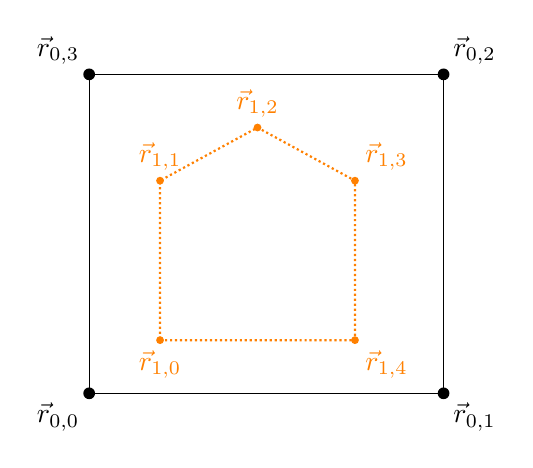
\begin{tikzpicture}[scale=2.25]
  \coordinate (zero) at (0, 0);
  \coordinate (one) at (2.0, 0);
  \coordinate (two) at (2.0, 1.8);
  \coordinate (three) at (0, 1.8);
  \draw
    (zero) node[below left] {$\vec{r}_{0,0}$}
    -- (one) node[below right] {$\vec{r}_{0,1}$}
    -- (two) node[above right] {$\vec{r}_{0,2}$}
    -- (three) node[above left] {$\vec{r}_{0,3}$}
    -- cycle;
  \foreach \n in {zero,one,two,three}
    \node at (\n)[circle,fill,inner sep=1.5pt]{};

  \coordinate (0) at (0.4, 0.3);
  \coordinate (1) at (1.5, 0.3);
  \coordinate (2) at (1.5, 1.2);
  \coordinate (3) at (0.95, 1.5);
  \coordinate (4) at (0.4, 1.2);
  \draw[orange,densely dotted,thick]
    (0) node[below] {$\vec{r}_{1,0}$}
    -- (1) node[below right] {$\vec{r}_{1,4}$}
    -- (2) node[above right] {$\vec{r}_{1,3}$}
    -- (3) node[above] {$\vec{r}_{1,2}$}
    -- (4) node[above] {$\vec{r}_{1,1}$}
    -- cycle;
  \foreach \n in {0,1,2,3,4}
    \node at (\n)[circle,fill,inner sep=1pt,orange]{};
\end{tikzpicture}

  \caption{%
    Simple polygon with four unique vertices is shown on the left hand side.
    A complex polygon with an outer hull
    and an interior hull is shown on the right hand side for comparison.
  }%
  \label{fig:polygon-representation}
\end{figure}

A polygon is considered invalid if one or more of its linear rings are self-intersecting, i.e.\ if any of its rings is considered to be complex.
Data providers frequently provide polygons in invalid states and such polygons must be corrected since they are often not processable by common GIS tools.
Zero-buffering invalid polygons (growing the polygon in all directions by zero units) fixes such problems, as can be seen in~\figref{fig:complex-zero-buffer}.

\begin{figure}[H]
  \centering
  \begin{tikzpicture}[scale=1]
  \coordinate (ll) at (0, 0);
  \coordinate (mid) at (2, 1);
  \coordinate (lr) at (4, 0);
  \coordinate (ur) at (4, 2);
  \coordinate (ul) at (0, 2);
  \draw[fill=orange]
    (ll) node[left] {$\vec{p}_0$}
    -- (ur) node[right] {$\vec{p}_1$}
    -- (lr) node[right] {$\vec{p}_2$}
    -- (ul) node[left] {$\vec{p}_3$}
    -- cycle;
  \foreach \n in {ll,ur,lr,ul}
    \node at (\n)[circle,fill,inner sep=1.5pt]{};

   \draw (4.4, 1) edge[->, thick] node[above] {\texttt{buffer(0.0)}} (6.6, 1);

  \coordinate (offset) at (7, 0);
  \draw[fill=orange]
    ($ (ll) + (offset) $) node[left] {$\vec{p}_0$}
    -- ($ (mid) + (offset) $) node[below] {$\vec{p}_1$}
    -- ($ (lr) + (offset) $) node[right] {$\vec{p}_2$}
    -- ($ (ur) + (offset) $) node[right] {$\vec{p}_3$}
    -- ($ (mid) + (offset) $) node[above] {$\vec{p}_4$}
    -- ($ (ul) + (offset) $) node[left] {$\vec{p}_5$}
    -- cycle;
  \foreach \n in {ll,mid,lr,ur,mid,ul}
    \node at ($ (\n) + (offset) $)[circle,fill,inner sep=1.5pt]{};
\end{tikzpicture}

  \caption{Illustration of how zero-buffering an invalid polygon corrects self-intersecting polygons.}%
  \label{fig:complex-zero-buffer}
\end{figure}

Zero-buffering polygons has the added benefit of normalizing vector data by re-ordering the polygon vertices in an anti-clockwise manner and removing redundant vertices as shown in~\figref{fig:redundant-zero-buffer}.

\begin{figure}[H]
  \centering
  \begin{tikzpicture}[scale=1]
  \coordinate (ll) at (0, 0);
  \coordinate (lm) at (2, 0);
  \coordinate (lr) at (4, 0);
  \coordinate (ur) at (4, 1);
  \coordinate (um) at (2, 1);
  \coordinate (Um) at (2, 2);
  \coordinate (ul) at (0, 1);
  \draw[fill=orange]
    (ll) node[below] {$\vec{r}_0$}
    -- (lm) node[below] {$\vec{r}_1$}
    -- (lr) node[below] {$\vec{r}_2$}
    -- (ur) node[above] {$\vec{r}_3$}
    -- (um) node[above right] {$\vec{r}_4$}
    -- (Um) node[above] {$\vec{r}_5$}
    -- (um) node[above left] {$\vec{r}_6$}
    -- (ul) node[above] {$\vec{r}_7$}
    -- cycle;
  \foreach \n in {ll,lm,lr,ur,um,Um,um,ul}
    \node at (\n)[circle,fill,inner sep=1.5pt]{};

   \draw (4.9, 0.5) edge[->, thick] node[above] {\texttt{buffer(0.0)}} (7.1, 0.5);

  \coordinate (offset) at (8, 0);
  \draw[fill=orange]
    ($ (ll) + (offset) $) node[below] {$\vec{r}_0$}
    -- ($ (lr) + (offset) $) node[below] {$\vec{r}_1$}
    -- ($ (ur) + (offset) $) node[above] {$\vec{r}_2$}
    -- ($ (ul) + (offset) $) node[above] {$\vec{r}_3$}
    -- cycle;
  \foreach \n in {ll,lr,ur,ul}
    \node at ($ (\n) + (offset) $)[circle,fill,inner sep=1.5pt]{};
\end{tikzpicture}

  \caption{Illustration of how zero-buffering polygons removes redundant vertices.}%
  \label{fig:redundant-zero-buffer}.
\end{figure}

This allows you to apply simpler similarity measures for comparing polygons, and reduces computational costs when processing the polygons.
Technical details for applying zero-buffers to vector data is provided in~\appref{app:zero-buffer}.
We will come back to how to combine vector and raster datasets by \textit{rasterization} in~\secref{sec:masking} where it will also become clear why the removal of redundant vertices is of importance.


\subsubsection{Raster data}
\label{sec:raster-data}
% \usepackage{tikz-3dplot}
% \tdplotsetmaincoords{60}{125}
% \tdplotsetrotatedcoords{0}{0}{0}

\begin{tikzpicture}[scale=3,tdplot_rotated_coords,
                    cube/.style={very thick,black},
                    grid/.style={very thin,gray},
                    axis/.style={->,ultra thick},
                    rotated axis/.style={->,purple,ultra thick}]

    \tikzmath{
      \gridspacing=0.25;
    }
    %draw a grid in the x-y plane
    \foreach \x in {-0.5,0,...,2.5}
        \foreach \y in {-0.5,0,...,2.5}
        {
            \draw[grid,blue,thick] (\x,-0.5,0) -- (\x,2.5,0);
            \draw[grid,blue,thick] (-0.5,\y,0) -- (2.5,\y,0);
        }

    \foreach \x in {-0.5,0,...,2.5}
        \foreach \y in {-0.5,0,...,2.5}
        {
            \draw[grid,green,thick] (\x,-0.5,\gridspacing) -- (\x,2.5,\gridspacing);
            \draw[grid,green,thick] (-0.5,\y,\gridspacing) -- (2.5,\y,\gridspacing);
        }

    \foreach \x in {-0.5,0,...,2.5}
        \foreach \y in {-0.5,0,...,2.5}
        {
            \draw[grid,red,thick] (\x,-0.5,2*\gridspacing) -- (\x,2.5,2*\gridspacing);
            \draw[grid,red,thick] (-0.5,\y,2*\gridspacing) -- (2.5,\y,2*\gridspacing);
        }

    %draw the main coordinate frame axes
    \draw[axis,tdplot_main_coords] (-1.5,-1.5,0) -- (-0.5,-1.5,0) node[anchor=west]{$x$};
    \draw[axis,tdplot_main_coords] (-1.5,-1.5,0) -- (-1.5,-0.5,0) node[anchor=north west]{$y$};
    \draw[axis,tdplot_main_coords] (-1.5,-1.5,0) -- (-1.5,-1.5,1) node[anchor=west]{$z$};

    \node[circle,radius=1,above] at (-0.5, -0.5, 2*\gridspacing) {$test$};
\end{tikzpicture}


\subsection{Data sets}

\subsubsection{LiDAR data}
\todo{Write about LiDAR data.}


\subsubsection{Building data}
\todo{
  Write about Trondheim building data set, provided in \\
  \texttt{Basisdata\_5001\_Trondheim\_5972\_FKB-Bygning\_GML.gml}.
}


\subsubsection{Summary of data sets}
\begin{table}[h]
  \centering
  \resizebox{\textwidth}{!}{%
    \begin{tabular}{lSSrrrr}
      \toprule
      {Data set} & {Resolution} & {Size} & {Coverage area} & {Date} & Scan angle & Accuracy \\
      \midrule
      Orthophoto \cite{trondheim_ortophoto_2017} & \SIrange{0.04}{0.15}{\meter} & \SI{161}{\giga\byte}  & TODO & \date{2017} & {} & \SI{\pm 0.35}{\meter} \\
      LiDAR \cite{trondheim_lidar_2017} & \SI{0.2}{\meter} & \SI{25}{\giga\byte} & \SI{342}{\kilo\meter\squared} & \date{2017-10-10} & \SI{\pm 20}{\degree} & \SI{\pm 0.02}{\meter} (SD) \\
      \bottomrule
    \end{tabular}%
  }
\end{table}

\begin{table}[h]
  \centering
  \begin{tabular}{cc}
    \toprule
    {Point density (\si{\per\meter\squared})} & {Proportion (\%)} \\
    \midrule
    $> 100\%$ & 97.7 \\
    \SIrange{85}{100}{\percent} & 1.2 \\
    \SIrange{60}{85}{\percent} & 1.1 \\
    \bottomrule
  \end{tabular}
  \caption{
    Control of point cloud density of the Trondheim 2017 LiDAR data set.
    The densities are calculated within rolling windows of size $\SI{10}{\meter} \times \SI{10}{\meter}$
    \cite{trondheim_lidar_2017}.
    }
\end{table}

